% author: Matheus Figueiredo

\documentclass {article}

\usepackage {tikz}
\usetikzlibrary {automata, positioning, arrows}

\begin{document}
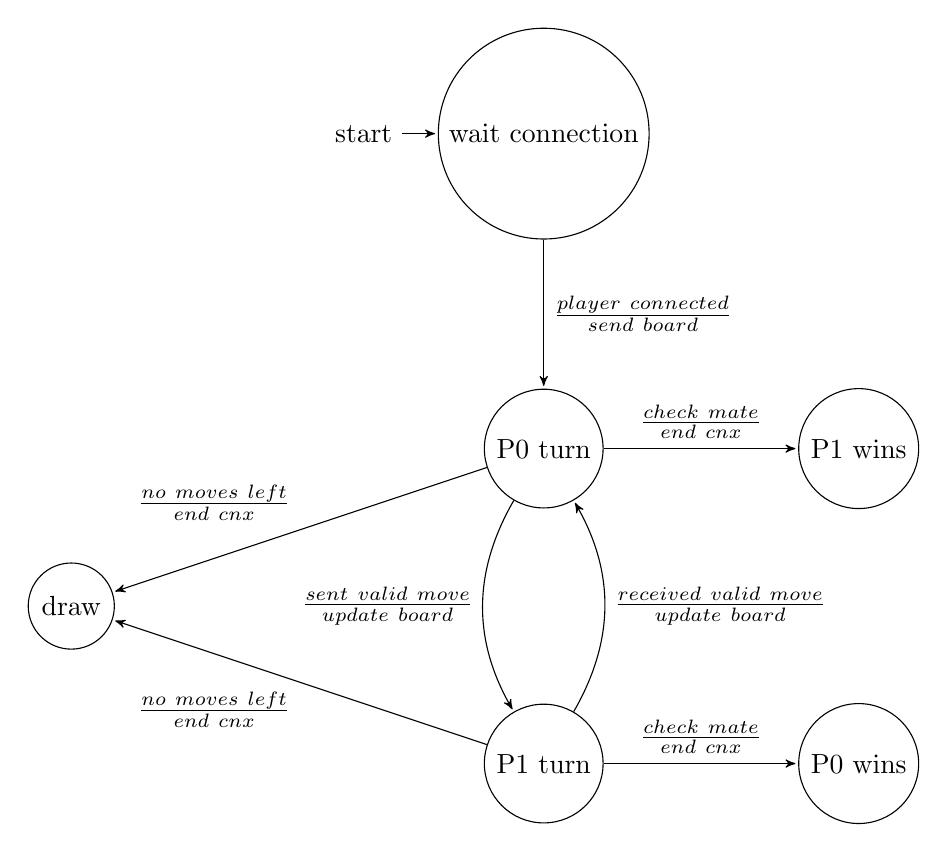
\begin{tikzpicture}[shorten >=1pt,node distance=4cm,on grid,auto]
  \tikzset{->, >=stealth'}
  
  \node[state,initial]  (q_0)                         {wait connection}; 
  \node[state]          (q_1) [below      = of q_0]   {P0 turn}; 
  \node[state]          (q_2) [below      = of q_1]   {P1 turn};
  \node[state]          (q_3) [right      = of q_1]   {P1 wins};
  \node[state]          (q_4) [right      = of q_2]   {P0 wins};
  \node[state]          (q_5) [below left = 2cm and 6cm of q_1] {draw};
  \path[->]
  % jesus cristo codigo feio do caralho
    (q_0) edge node {$\frac{player\ connected}{send\ board}$} (q_1)
    (q_1) edge [bend right] node [swap] {$\frac{sent\ valid\ move}
                                        {update\ board}$} (q_2)
          edge node [swap] {$\frac{no\ moves\ left}{end\ cnx}$} (q_5)
          edge node {$\frac{check\ mate}{end\ cnx}$} (q_3)
    (q_2) edge [bend right] node [swap] {$\frac{received\ valid\ move}
                                        {update\ board}$} (q_1)
          edge node {$\frac{no\ moves\ left}{end\ cnx}$} (q_5)
          edge node {$\frac{check\ mate}{end\ cnx}$} (q_4);
\end{tikzpicture}
\end{document}  
